\documentclass{beamer}

% tout le bazar jusqu'à title, c'est du chinois beamer/pdf illisible...

% importations de packages utiles
\usepackage[utf8]{inputenc}  % pouvoir écrire avec des accents
\usepackage[french]{babel}  % francophopnie
\usepackage{hyperref}  % liens clicables dans pdf final
\usepackage{tikz}  % pouvoir tracer des dessins sympas
\usetheme{Boadilla}  % thème de beamer
\usepackage{listingsutf8}  % rendu de "code" (avec config ci-dessous)
\definecolor{lstcolor}{rgb}{0.9,0.95,0.95}
\definecolor{lstcommentcolor}{rgb}{0.,0.2,0.}
\lstset{
  frameround=tttt,
  %autogobble,
  frame=single,
  backgroundcolor=\color{lstcolor},
  % extendedchars=true,
  % basicstyle=\ttfamily\small,
  keywordstyle=\bfseries\color{blue},
  identifierstyle=\bfseries\color{red},
  stringstyle=\bfseries\color{orange},
  commentstyle=\color{lstcommentcolor},
  language=Python,
  keepspaces=True,
  basicstyle=\fontfamily{pcr}\selectfont\small, % monospace it for copypasting
  upquote=true,
  columns=flexible,
  showstringspaces=False,
  literate={é}{{\'e}}1
}
\usepackage{array}
\title{Projet \textit{RNG}}
\subtitle{Algorithmes et Structures de Données II}
\author{Juan-Carlos Barros, Yves Dethurens,\\ Daniel Kessler et Jean-Francis Ravoux}
% et c'est parti
\begin{document}
\begin{frame}
  \titlepage
\end{frame} % titre
\begin{frame}
  \tableofcontents
\end{frame} % toc

\begin{frame}{Dans quels domaines a-t-on des nombres aléatoires?}
  \begin{tabular}{m{.45\textwidth}m{.4\textwidth}}
  
\includegraphics[width=.4\textwidth]{img/rng_gaming.png}&
  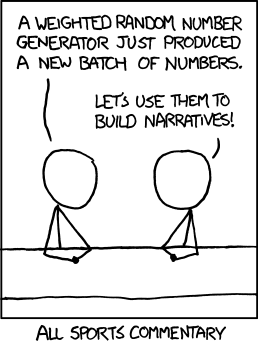
\includegraphics[width=.25\textwidth]{img/xkcd_sports.png}
  \end{tabular}\par
  
\includegraphics[width=.8\textwidth]{img/dilbert_financial.png}
  \end{frame}

\section{Distributions}
\begin{frame}
  \frametitle{Distributions aléatoires discrètes}
  \begin{itemize}
  \item $f(x)$, la ``fréquence'' de $x$, est la probabilité de tirer $x$.
  \item $f(x)\geq0, \;\forall x$
  \item $\sum_xf(x)=1$
  \end{itemize}
  \begin{tabular}{ccc}
    \onslide<2->{
    \begin{tikzpicture}[scale=.5, every node/.style={scale=0.5}]
      \draw[->] (-.2,0) -- (5.5,0) node[right] {$x$};
      \draw[->] (0, -0.2) -- (0, 4.2) node[above] {$f(x)$};
      \foreach \i in {1, ..., 5} {
        \draw[blue] (\i, 0) -- (\i, 3.5);
        \node at (\i, -0.3) {$\i$};
      }
      \draw (.1, 3.5) -- (-.1, 3.5) node[left] {$0.2$};
    \end{tikzpicture}}
    &\onslide<3->{
      \begin{tikzpicture}[scale=.5, every node/.style={scale=0.5}]
        \draw[->] (-1.2,0) -- (5.2,0) node[right] {$x$};
        \draw[->] (-1,-0.2) -- (-1,6.2) node[above] {$f(x)$};
        \draw[blue] (0, 0) -- (0, 1);
        \draw[blue] (1, 0) -- (1, 4);
        \draw[blue] (2, 0) -- (2, 6);
        \draw[blue] (3, 0) -- (3, 4);
        \draw[blue] (4, 0) -- (4, 1);
        \foreach \i in {0, ..., 5} {
          \node[below] at (\i, 0) {$\i$};
        }
      \end{tikzpicture}}
    &\onslide<4->{
      \begin{tikzpicture}[scale=.5, every node/.style={scale=0.5}]
        \draw[->] (-1.2,0) -- (4.2,0) node[right] {$x$};
        \draw[->] (-1,-0.2) -- (-1,4.2) node[above] {$f(x)$};
        \node[blue] at (1.5, 2) {\Huge ?};
      \end{tikzpicture}}
    \\
    \onslide<2->{uniforme} & \onslide<3->{binômiale} & \onslide<4->{autre}
  \end{tabular}    
\end{frame}
\begin{frame}
  \frametitle{Distributions aléatoires continues}
  \begin{itemize}
  \item $\int_a^bf(x)$ est la probabilité de tirer $x$ entre $a$ et $b$.
  %\item $f(x)\geq0, \;\forall x$
  \item $\int_{-\infty}^{+\infty}f(x)=1$
  \end{itemize}
  \begin{tikzpicture}
    \draw[->] (-.2,0) -- (4.2,0) node[right] {$x$};
    \draw[->] (0,-0.2) -- (0,2.2) node[above] {$f(x)$};
    \draw[blue] (1, 0) -- (1, 1) -- (3, 1) -- (3, 0);
    \draw (1, .1) -- (1, -.1) node[below] {\small$c$};
    \draw (3, .1) -- (3, -.1) node[below] {\small$d$};
    \node at (2, 2.2) {uniforme};
    \onslide<2->{
    \def\dx{6.8}; \def\dy{-3};
    \draw[->] (-4.2+\dx, \dy) -- (4.2+\dx,\dy) node[right] {$x$};
    \draw[->] (\dx-1,\dy-.2) -- (\dx-1, 2.2+\dy) node[above] {$f(x)$};
    \draw[blue] (\dx, \dy) plot[domain=-4:4, samples=200] ({\x+\dx},{\dy+2*2^(-\x*\x)});
    \draw (\dx, .1+\dy) -- (\dx, \dy-.1) node[below] {\small$\mu$};
    \def\ec{1.3}
    \draw (\dx+\ec, .1+\dy) -- (\dx+\ec, \dy-.1) node[below] {\small$\mu+\sigma$};
    \draw (\dx-\ec, .1+\dy) -- (\dx-\ec, \dy-.1) node[below] {\small$\mu-\sigma$};
    \node at (\dx+1, \dy+2.3) {normale};
    }\onslide<3->{
    \def\dx{8}; \def\dy{.5};
    \draw[->] (\dx-.2, \dy) -- (\dx+3.2,\dy) node[right] {$x$};
    \draw[->] (\dx-.1,\dy-.2) -- (\dx-.1, \dy+2.2) node[above] {$f(x)$};
    \node[blue] at (\dx+1.5, \dy+1) {\Huge ?};
    \node at (\dx+1.5, \dy+2.2) {autre};
    }
  \end{tikzpicture}
\end{frame}
\begin{frame}
  \frametitle{Génération de nombres aléatoires}
  \begin{center}
    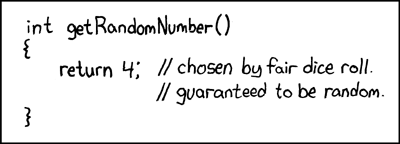
\includegraphics[width=.6\textwidth]{img/xkcd_fair.png}\par
    (source: xkcd.com)
  \end{center}
\end{frame}

\section{Exemple pour Jean-Francis}
\begin{frame}{Exemple pour Jean-Francis}
  \begin{minipage}{0.32\textwidth}
    \onslide<1->{Du texte inutile gauche\par}
    \onslide<2->{Du texte inutile en plus}
  \end{minipage}
  \begin{minipage}{0.33\textwidth}
    Du texte inutile central
  \end{minipage}
  \begin{minipage}{0.32\textwidth}
    \only<1-2>{Du texte inutile droit}
    \only<3->{Un texte différent}
  \end{minipage}
  
\end{frame}

\section{``vrai'' ou ``pseudo''-aléatoire?}
\begin{frame}
  \frametitle{``vrai'' ou ``pseudo''-aléatoire?}
  \ldots Telle est la question!
\end{frame}

\section{Générateurs de suites pseudo-aléatoires}
\begin{frame}
  \frametitle{Générateurs de suites pseudo-aléatoires}
\end{frame}

\section{Comment produire un ``seed''?}
\begin{frame}
  \frametitle{Comment produire un ``seed''?}
\end{frame}

\section{Que fait le module ``random'' de Python?}
\begin{frame}
  \frametitle{Que fait le module ``random'' de Python?}
\end{frame}

\section{Générateurs de suites ``vraiment'' aléatoires}
\begin{frame}
  \frametitle{Générateurs de suites ``vraiment'' aléatoires}
  \ldots quantique \ldots
\end{frame}
\end{document}
